% Name: Pushdown automaton
% Description: A PDA that accepts aⁿbⁿ: it pushes on a, pops on b, and accepts when the stack is back to Z.
% Tags: PDA, pushdown automaton, context-free language

\usetikzlibrary{automata, positioning, arrows.meta}

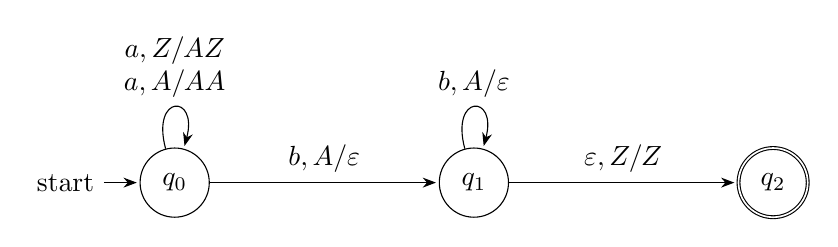
\begin{tikzpicture}[shorten >=1pt, node distance=3.8cm, on grid, auto, >={Stealth}]
  \node[state, initial] (q0) {$q_0$};
  \node[state] (q1) [right=of q0] {$q_1$};
  \node[state, accepting] (q2) [right=of q1] {$q_2$};

  \path[->]
    (q0) edge[loop above] node[align=center] {$a, Z / AZ$\\$a, A / AA$} ()
         edge node {$b, A / \varepsilon$} (q1)
    (q1) edge[loop above] node {$b, A / \varepsilon$} ()
         edge node {$\varepsilon, Z / Z$} (q2);
\end{tikzpicture}
